\chapter{Integracija računalnog oblaka i razvojnog sustava}

Ovo poglavlje opisuje biblioteke i primjere korištenje za povezivanje modula ESP32-C3 s računalnim oblakom AWS sustava. Za početno povezivanje korištena je demo aplikacija koja automatski povezuje razvojni sustav s \textit{backend} dijelom AWS sustava. U idućim poglavljima korištene su razne biblioteke za povezivanje uređaja i oblaka.

\section{Probno povezivanje korištenjem demo aplikacije AWS \textit{Quick Connect}}

Za početno probno povezivanje razvojnog sustava ESP32-C3 sa sustavom AWS, korištena je službena demo aplikacija \textit{Quick Connect} projekta \textit{FreeRTOS}, koji je trenutno u vlasništvu AWS-a. Ova aplikacija, nakon učitavanja binarne datoteke u razvojni sustav i definiranje vjerodajnica za povezivanje na Wi-Fi, putem protokola MQTT šalje informacije s uređaja u AWS \cite{quick_connect_app}. Račun za uređaj se automatski stvori te nije potrebna nikakva dodatna prijava u sam sustav. Na slici \ref{fig:aws_esp32_easy_connect} nalazi se ispis u konzoli nakon što se pokrene demo aplikacija na razvojnom sustavu. Iz slike je vidljivo postavljanje (engl. \textit{provisioning}) uređaja, kao i kreiranje certifikata za siguran prijenos podataka.

\begin{figure}[ht]
	\centering
	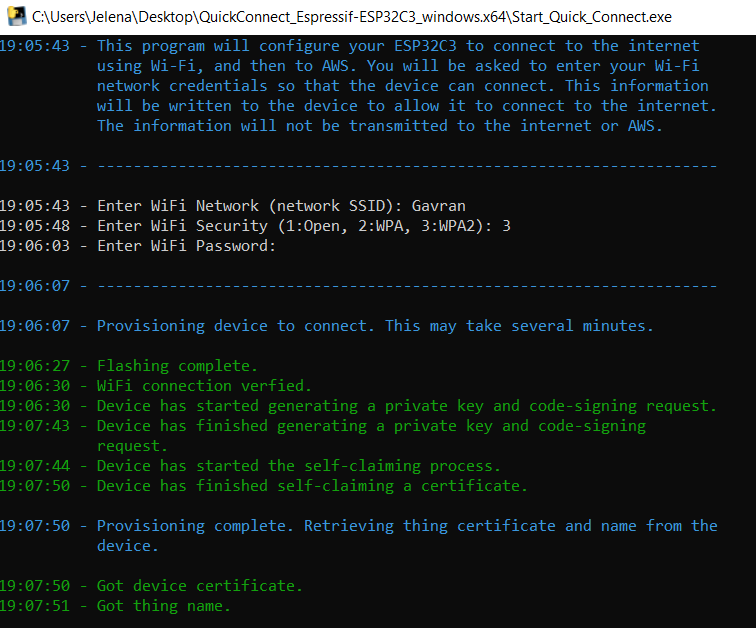
\includegraphics[scale=0.6]{imgs/aws_esp32_easy_connect}
	\caption{Ispis u konzoli pri pokretanju demo aplikacije Quick Connect}
	\label{fig:aws_esp32_easy_connect}
\end{figure}

Slika \ref{fig:esp32_easy_connect_mqtt_packages} također prikazuje ispis u konzoli, no ovaj puta sadržaj paketa koji se šalju protokolom MQTT. Podaci su prikazani u formatu JSON.

\begin{figure}[ht]
	\centering
	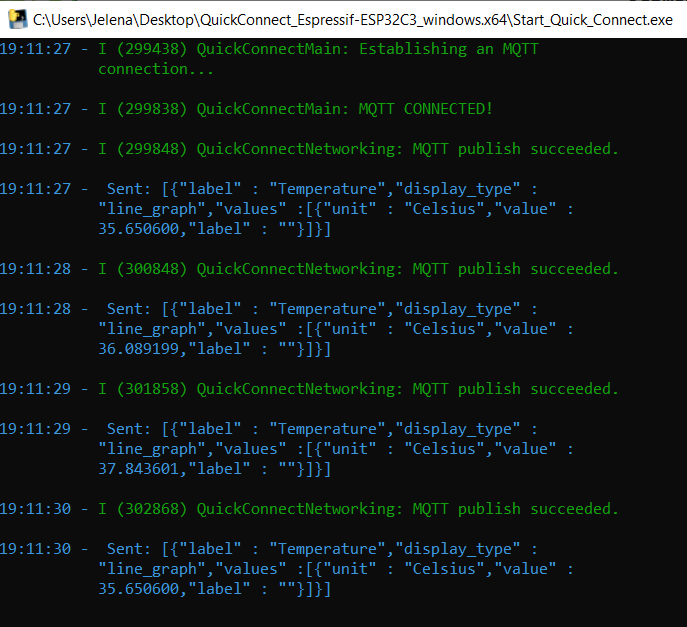
\includegraphics[scale=0.6]{imgs/esp32_easy_connect_mqtt_packages}
	\caption{Ispis slanja paketa protokolom MQTT s razvojnog sustava ESP32-C3}
	\label{fig:esp32_easy_connect_mqtt_packages}
\end{figure}

Iako je demo primjer uspješno slao podatke putem MQTT protokola, podaci se nisu prikazivali na stranici. Slika \ref{fig:no_or_slow_data} prikazuje stranicu projekta \textit{FreeRTOS} te identifikacijski broj uređaja koji se spojio, no sami podaci koje uređaj šalje nisu prikazani budući da nisu ni primljeni. Nije provođeno daljnje otklanjanje pogrešaka jer je ova aplikacija pružena \textit{out-of-the-box}, te za detaljniju analizu problema potrebno je prolaziti kroz izvorni kod aplikacije. Stoga su odabrana druga rješenja za povezivanje razvojnog sustava s uslugama AWS-a.

%\begin{figure}[ht]
%	\centering
%	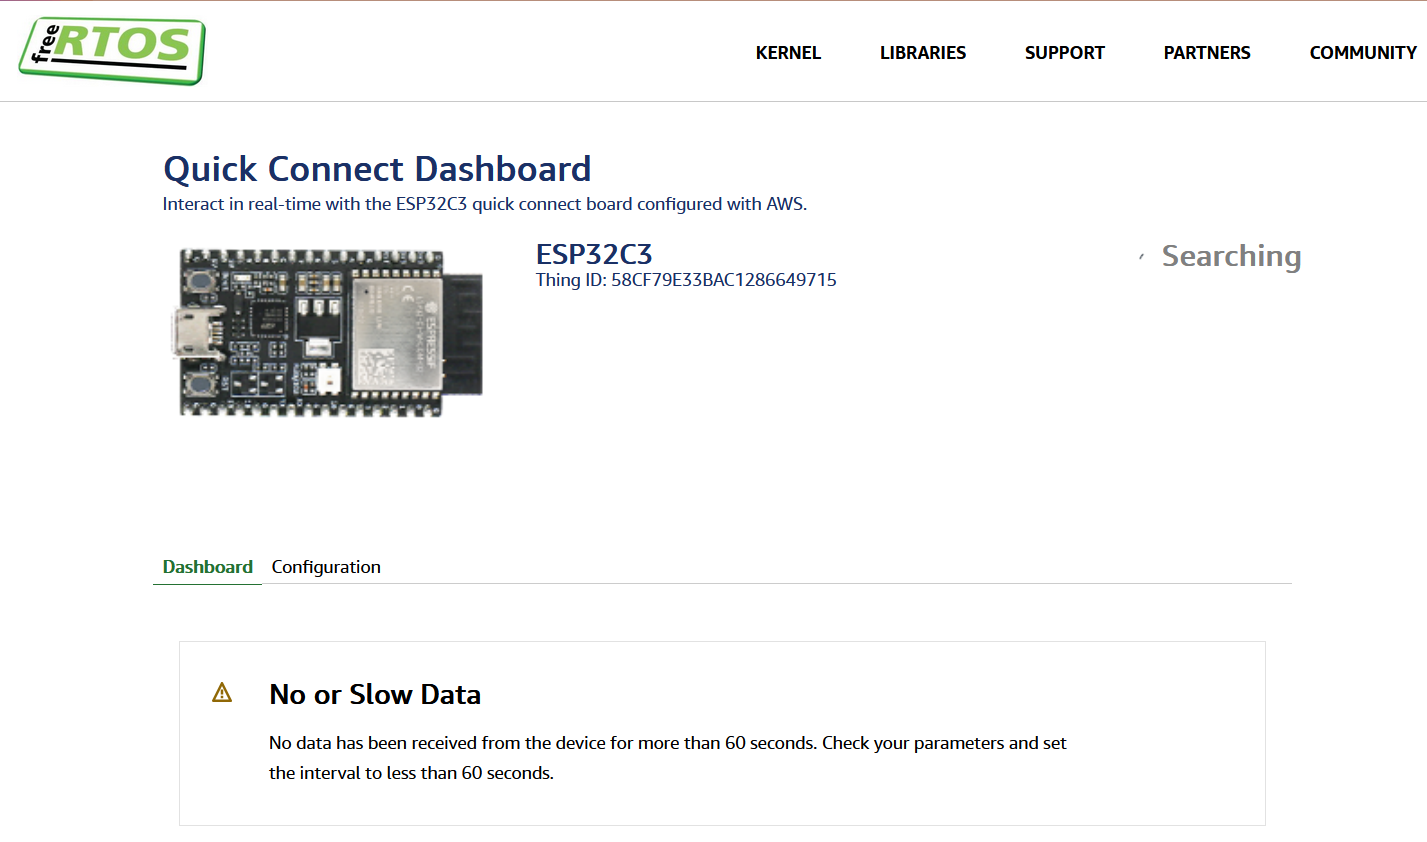
\includegraphics[scale=0.5]{imgs/no_or_slow_data}
%	\caption{Stranica projekta \textit{FreeRTOS} s prikazom spojenog razvojnog sustava ESP32-C3}
%	\label{fig:no_or_slow_data}
%\end{figure}

\section{Biblioteka \textit{esp-aws-iot}} 

Kao drugi primjer korištena je biblioteka \textit{esp-aws-iot} \cite{esp-aws-iot}, koja također sadrži gotove primjere za povezivanje sa sustavom AWS. U nastavku su navedene glavne značajke koje biblioteka podržava:
\begin{enumerate}
	\item \textit{Fleet Provisioning} - usluga koju nudi AWS, a odnosi se na konfiguriranje uređaja u oblaku bez unaprijed definiranih certifikata,
	\item \textit{Thing Shadow} - ranije opisane sjene stvarnih uređaja,
	\item poslovi (engl. \textit{jobs}) - akcije koje se mogu izvršiti na samom uređaju ili u oblaku,
	\item OTA (engl. \textit{Over The Air}) - podržava ažuriranje postavki i koda uređaja putem mreže, podržani protokoli HTTP i MQTT, 
	\item HTTP povezivanje,
	\item MQTT povezivanje.
\end{enumerate}

OTA ažuriranje uređaja vrlo je moćna značajka koja ne zahtijeva ponovni unos koda na uređaj, nego se mrežnim putem ažuriraju željene značajke i tako izmijeni izvorni kod. Biblioteka i AWS primarno podržavaju protokol MQTT za OTA prijenos, no eksperimentalno je omogućen i protokol HTTP, upravo jer nema razinu sigurnosti koja je pružena protokolom MQTT.

Ova biblioteka koristi mogućnosti koje pruža usluga AWS IoT Core za povezivanje s fizičkim uređajima. Prije pokretanja primjera na samom uređaju, potrebno je napraviti AWS račun za korisnika, te mu dodijeliti potrebna prava i politike. Isto tako, kako bi se uređaj spojio na AWS koristeći protokol TLS za sigurno povezivanje, potrebno je generirati i sigurnosne certifikate. Kako bi uređaj komunicirao s oblakom, potrebno ga je registrirati u sustavu AWS. Pri stvaranju odnosno registraciji pojedine \textit{Stvari}, generiraju se i certifikati koji je zatim potrebno učitati u memoriju uređaja. Ovaj korak nije nužan ako se uređaj spaja putem usluge \textit{Fleet Provisioning}. 

Generirana sigurnosna politika daje dozvolu za sljedeće radnje:
\begin{itemize}
	\item povezivanje - dopušta uređaju povezivanje na brokera u oblaku s bilo kojim klijentskim identifikatorom, 
	\item objava poruka - uređaj može objavljivati poruke protokolom MQTT na bilo koju temu,
	\item pretplata na teme - moguća je pretplata na bilo koju temu u brokeru,
	\item prihvat poruka - uređaj može primati poruke od brokera s bilo koje teme.
\end{itemize}

Detaljniji koraci stvaranja računa, prava i potrebnih certifikata mogu se pronaći ovdje \cite{setup_aws}.

Ova je biblioteka korištena za povezivanje uređaja na AWS broker. Korišten je testni broker dostupan u sklopu usluge AWS IoT Core. Povezivanje na internet u ovom primjeru omogućeno je programatski, te je potrebno unaprijed definirati vjerodajnice Wi-Fi veze. Uređaj je, povezavši se na internet i broker pomoću ranije generiranih certifikata, kontinuirano slao testnu poruku na broker. Prikaz poruka koje je broker primio na testnu temu nalazi se na slici \ref{fig:testClient_helloworld}. Budući da nije postavljen način parsiranja poruka, javlja se greška, iako su poruke uredno prikazane.

\begin{figure}[ht]
	\centering
	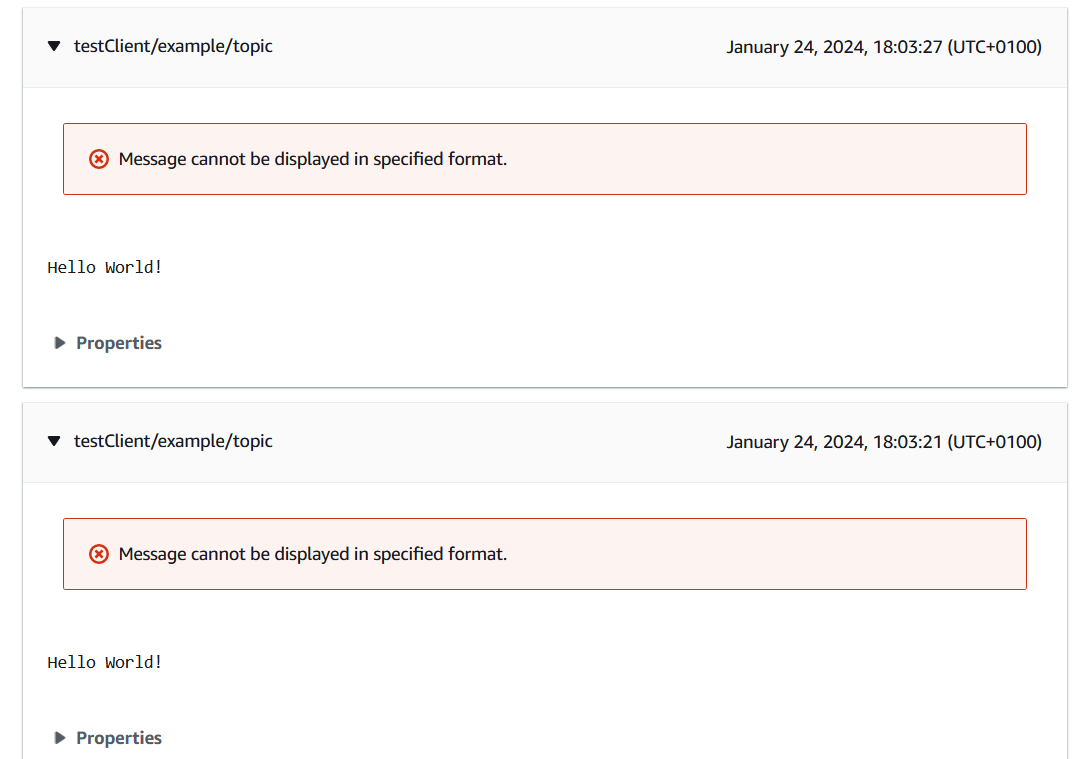
\includegraphics[scale=0.5]{imgs/testClient_helloworld}
	\caption{Ispis poruke u AWS brokeru na temu \textit{testClient/example/topic}}
	\label{fig:testClient_helloworld}
\end{figure}

\section{Programski paket \textit{iot-reference-esp32c3}} 

Ovaj programski paket \cite{iot-reference-esp32-c3} proširenje je prethodno opisane biblioteke, te integrira više njezinih značajki za potpun prikaz mogućnosti koje biblioteka nudi. 

Paket podržava tri demo simulacije implementirane kao tri FreeRTOS zadaće, od kojih svaka koristi istu MQTT vezu. Simulacije koriste biblioteku \textit{coreMQTT}, dok se biblioteka \textit{coreMQTT-Agent} koristi radi osiguranja pouzdane međudretvenosti unutar MQTT konekcije. Simulacije su sljedeće:

\begin{itemize}
	\item \textit{ota\_over\_mqtt\_demo}: praćenje OTA ažuriranja putem protokola MQTT,
	\item \textit{sub\_pub\_unsub\_demo}: Kružna pretplata i odjava s tema u brokeru također koristeći protokol MQTT,
	\item \textit{temp\_sub\_pub\_and\_led\_control\_demo}: Objava poruka i kontroliranje LED lampice na uređaju.
\end{itemize}

Simulacija \textit{ota\_over\_mqtt\_demo} koristi OTA uslugu koju nudi AWS u sklopu FreeRTOS projekta za konfiguriranje i kreiranje OTA ažuriranja. OTA klijentski softver na razvojnom sustavu koristi AWS IoT OTA biblioteku i u pozadini je vrti unutar FreeRTOS zadatka. Simulacija se pretplati i sluša na temi zaduženoj za OTA ažuriranja. Po primitku obavijesti o nadolazećem ažuriranju, preuzima novu verziju i potvrđuje potpis preuzetog ažuriranja certifikatom. Po uspješnoj verifikaciji, uređaj se resetira i aktivira se nova verzija.  

Zadaci unutar simulacije \textit{sub\_pub\_unsub\_demo} pretplaćuju se na temu u oblaku AWS IoT Core, šalju konstantan string na istu temu na koju su pretplaćeni, te se zatim odjave s teme, te tako u krug.

Simulacija \textit{temp\_sub\_pub\_and\_led\_control\_demo} kreira zadatak koji se pretplati na temu unutar oblaka AWS IoT Core. Zatim se čita temperatura sa senzora za temperaturu integriranog u modul te se objavljuje u formatu JSON na istu temu na koju je i pretplaćen. Također, omogućava korisniku primanje paketa za paljenje ili gašenje LED lampice. 

Sve tri demo zadaće mogu se paralelno izvršavati kao odvojeni zadaci.

Glavna značajka koju koristi ovaj paket jest da se povezivanje na Wi-Fi mrežu odvija pomoću BLE tehnologije. Wi-Fi mreža konfigurira se putem sigurnosnih sesija uspostavljenih Bluetooth kanalom, i tako uklanja potrebu za upisivanjem vjerodajnica direktno u programski kod. Razvojni sustav pri pokretanju generira QR kod koji je potrebno skenirati mobilnom aplikacijom koju nudi tvrtka \textit{Espressif} \cite{esp_ble_provisioning} kako bi se uređaj povezao na mrežu. Uređaj, tako jednom spojen na mrežu, nema potrebe ponovno se spajati pri svakom uključivanju i isključivanju jer se vjerodajnice zapisuju u memoriju. Jedino brisanjem particije NVS (engl. \textit{Non-Volatile Storage}) memorije tipa \textit{Flash} moguće je spojiti se na novu Wi-Fi mrežu. 

Na slici \ref{fig:ocean_koda} nalazi se ispis u konzoli s modula kada se pokrenu sve tri simulacije odjednom. Crvenom su bojom istaknuti zadaci koje logiraju informativne poruke, dok je narančastom bojom istaknut zadatak koji šalje podatkovni paket u JSON formatu protokolom MQTT. Budući da razvojni sustav nema integrirani temperaturni senzor, vrijednost koja bi trebala biti očitana postavlja se na nulu. Na slici \ref{fig:kilometarski_primjer} prikazan je taj podatak (ali u drugoj iteraciji slanja) u brokeru unutar sustava AWS.

\begin{figure}[ht]
	\centering
	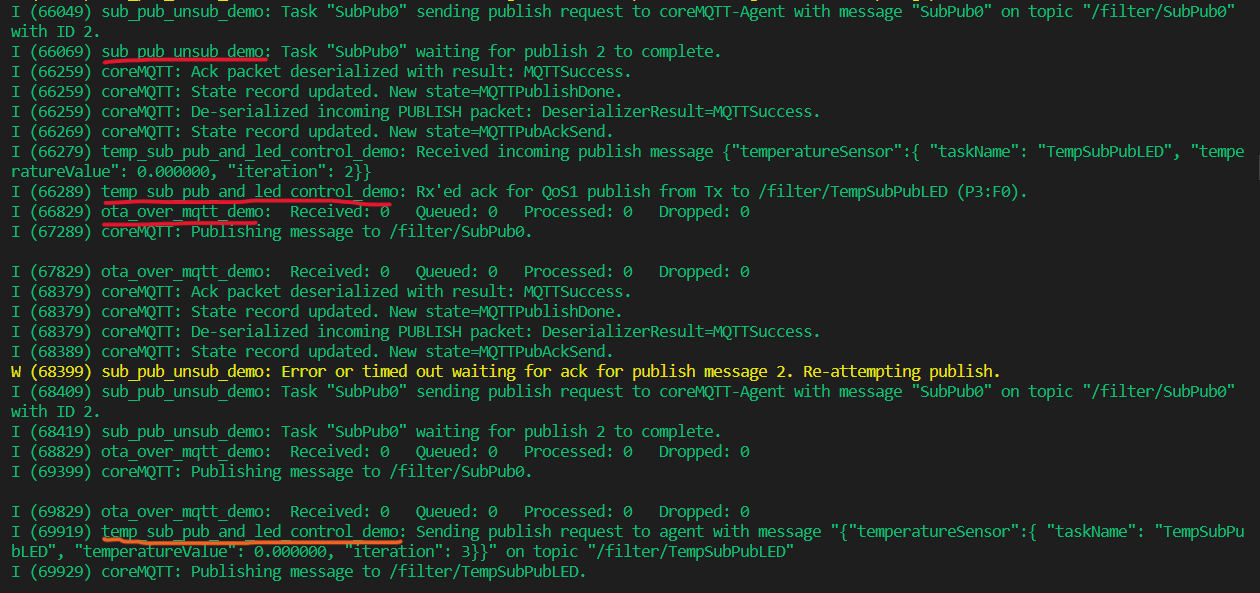
\includegraphics[scale=0.5]{imgs/ocean_koda}
	\caption{Ispis u konzoli s modula ESP32-C3}
	\label{fig:ocean_koda}
\end{figure}

\begin{figure}[ht]
	\centering
	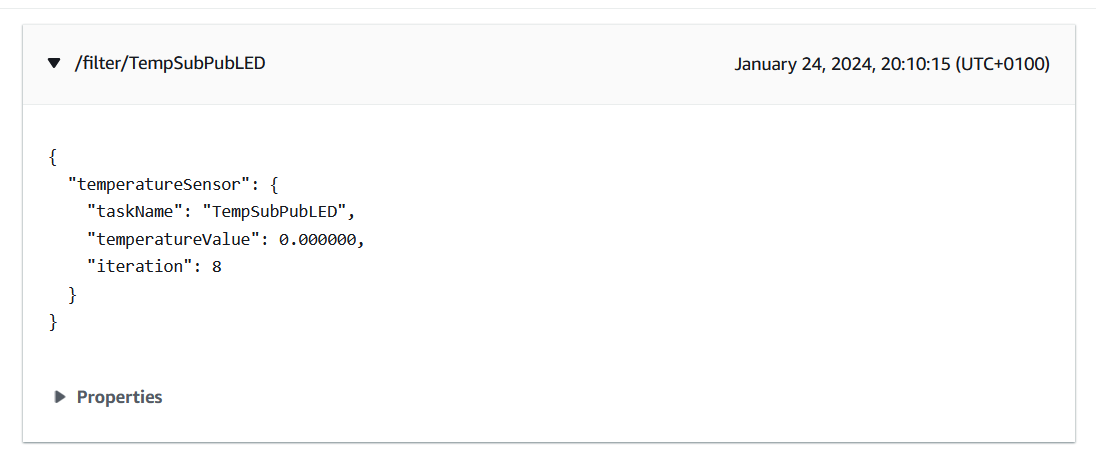
\includegraphics[scale=0.5]{imgs/kilometarski_primjer}
	\caption{Poruka na AWS brokeru}
	\label{fig:kilometarski_primjer}
\end{figure}

Radi manje pokazne simulacije stvarnog IoT sustava koji bi koristio opisane integrirane tehnologije, u sustav je priključen modul DHT11 koji vraća digitalni izlaz proporcionalan temperaturi i vlagi. Za čitanje podataka sa senzora korištena je službena biblioteka tvrtke \textit{Espressif} u okvir radnog okvira ESP-IDF koja nudi upravljački program za korištenje modula DHT11. Uklonjena je simulacija za OTA ažuriranje, te su ostavljene druge dvije vezane za MQTT brokera. Izmijenjen je dio programskog koda koji koristi integrirani temperaturni senzor kako bi se koristio novospojeni modul. 

Slika \ref{fig:komadic_outputa} tako prikazuje dio ispisa konzole, te ne postoji oznaka za OTA ažuriranje budući da taj posao nije pokrenut. Isto tako, vidljivo je da paket koji se šalje ima temperaturu postavljenu na ne-nul vrijednost, nego stvarnu temperaturu prostora u kojem se modul nalazi. 

\begin{figure}[ht]
	\centering
	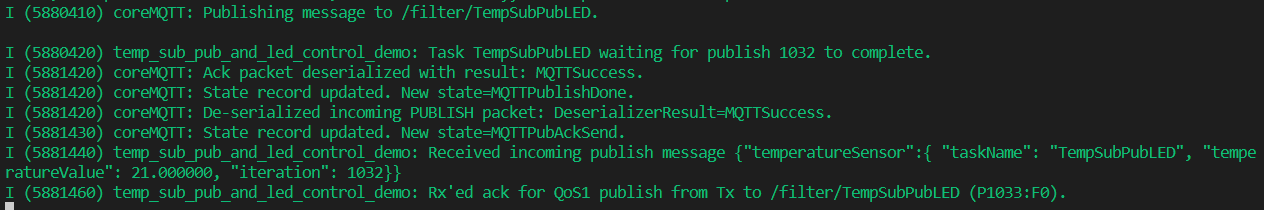
\includegraphics[scale=0.5]{imgs/komadic_outputa}
	\caption{Ispis u konzoli s modula ESP32-C3 spojenog s DHT11}
	\label{fig:komadic_outputa}
\end{figure}


\section{Buduća razmatranja}

Ranije opisane biblioteke i programski paketi nude paletu mogućnosti rada s razvojnim sustavom ESP32-C3 te mnoštvo značajki za integraciju sa uslugom AWS. Jedna od značajki koju je potrebno uzeti u obzir prilikom izrade budućeg stvarnog IoT sustava jest povezivanje uređaja u Wi-Fi mrežu. Kao što je opisano, biblioteke nude gotova rješenja za taj problem, omogućujući spajanje putem QR koda. Prvotni primjer, \textit{Quick Connect}, također dinamički unosi vjerodajnice u uređaj tako što se ručno upisuju kada se sustav pokreće. Idealan sustav bi imao zlatnu sredinu ova dva sustava - pri svakom pokretanju sustava da nije potrebno unositi Wi-Fi vjerodajnice, no isto tako da nije potrebna dodatna mobilna aplikacija za prijavu uređaja na mrežu. 

Nadalje, u korištenoj biblioteci te programskom kodu postoji mogućnost korištenja biblioteke za binarnu serijalizaciju podataka koji se šalju putem protokola MQTT. Format CBOR (engl. \textit{Concise Binary Object Representation}), za razliku od formata JSON, pretvara podatke u binarni oblik te ih tako šalje mrežom, što rezultira manjom latencijom i nosivošću (engl. \textit{payload}) \cite{cbor}. Pri prijenosu velike količine podataka pri ograničenim resursima, poput u IoT sustava, ušteda na veličini poslanih podataka znatno utječe na efikasnost sustava. Isto tako, binaran je format prilagodljiv u odnosu na JSON, gdje mora postojati unaprijed definirana shema za primitak podataka. Iduće iteracije sustava trebale bi razmotriti korištenje binarne serijalizacije radi poboljšanih performansi. 

\eject